\documentclass{harvardml}
\usepackage{graphicx}

% Authors: 
% Edited by: Mark Goldstein + others (jan 2018)
% Edited by: Amir Shanehsazzadeh, Andrew Kim, Nari Johnson (Jan 2021)
% Edited by: Max Guo, Raphael Pellegrin, Katherine Tian (Jan 2022)
% Edited once more by: William Tong (Jan 2023) + Skyler Wu (Jan 2023)
% Edited once more by: Jeffrey Xu (Jan 2024) + Gabriel Sun (Jan 2024)

% Adapted from CS281 Fall 2019 section 0 notes

% This tex file relies on
% the presence of two files:
% harvardml.cls and common.sty

\course{CS181-s24}
\assignment{Homework \#0}
\duedate{January 26, 2024 at 11:59 PM}

\usepackage{comment}
\usepackage{url}
\usepackage{float}
\usepackage{amsfonts, amsmath, amsthm}
\usepackage{listings}
\usepackage[shortlabels]{enumitem}
\usepackage{hyperref}
\usepackage{etoolbox}
\usepackage{color}

\theoremstyle{definition}
\newtheorem{defn}{Definition}[section]
\theoremstyle{plain}
\usepackage[textsize=tiny]{todonotes}

% Some useful macros.
\newcommand{\given}{\,|\,}
\newcommand{\R}{\mathbb{R}}
\newcommand{\C}{\mathbb{C}}
\newcommand{\E}{\mathbb{E}}
\newcommand{\var}{\text{Var}}
\newcommand{\cov}{\text{Cov}}
\newcommand{\p}{\partial}
\newcommand{\mba}{\mathbf{a}}
\newcommand{\mbb}{\mathbf{b}}
\newcommand{\mbx}{\mathbf{x}}
\newcommand{\mcX}{\mathcal{X}}
\newcommand{\mcY}{\mathcal{Y}}
\newcommand{\boldw}{\mathbf{w}}
\newcommand{\mbxt}{\tilde{\mathbf{x}}}
\newcommand{\Sigmat}{\tilde{\Sigma}}
\newcommand{\mbz}{\mathbf{z}}
\newcommand{\mbw}{\mathbf{w}}
\newcommand{\mcN}{\mathcal{N}}
\newcommand{\mcP}{\mathcal{P}}
\newcommand{\eps}{\epsilon}
\newcommand{\trans}{\intercal}
\newcommand{\Ut}{\tilde{U}}
\DeclareMathOperator*{\argmax}{arg\,max}
\newcommand{\angstrom}{\textup{\AA}}
\renewcommand{\v}[1]{\mathbf{#1}}


\usepackage{xcolor}
\newcount\Comments  % 0 suppresses notes to selves in text
\Comments = 1
\newcommand{\kibitz}[2]{\ifnum\Comments=1{\color{#1}{#2}}\fi}
\newcommand{\dcp}[1]{\kibitz{blue}{[DCP: #1]}}


% Solution environment
\newenvironment{solution}
  {\color{blue}\section*{Solution}}
{}


\begin{document}


\noindent Welcome to CS181! The purpose of this assignment is to help assess your readiness for this course.  It will be graded for completeness and effort.  \textbf{Areas of this assignment that are difficult are an indication of areas in which \emph{you} need to self-study. During the term, the staff will be prioritizing support for new material taught in CS181 over teaching prerequisites.}

\begin{enumerate}
    \item Please type your solutions after the corresponding problems using this \LaTeX\ template, and start each problem on a new page.
    \item Please submit the \textbf{writeup PDF to the Gradescope assignment `HW0'}. Remember to assign pages for each question.
    \item Please submit your \textbf{\LaTeX\ file and code files (i.e., anything ending in \texttt{.py}, \texttt{.ipynb}, or \texttt{.tex}) to the Gradescope assignment `HW0 - Supplemental'}. 
\end{enumerate}

\newpage
\begin{problem}[Modeling Linear Trends - Linear Algebra Review]
In this class we will be exploring the question of ``how do we model the trend in a dataset" under different guises. In this problem, we will explore the algebra of modeling a linear trend in data. We call the process of finding a model that capture the trend in the data, ``fitting the model."\\

\noindent \textbf{Learning Goals:} In this problem, you will practice translating machine learning goals (``modeling trends in data") into mathematical formalism using linear algebra. You will explore how the right mathematical formalization can help us express our modeling ideas unambiguously and provide ways for us to analyze different pathways to meeting our machine learning goals.\\

\noindent Let's consider a dataset consisting of two points $\mathcal{D} = \{(x_1, y_1), (x_2, y_2)\}$, where $x_n, y_n$ are scalars for $n=1, 2$. Recall that the equation of a line in 2-dimensions can be written: $y = w_0 + w_1x$. 
\begin{enumerate}
    \item Write a system of linear equations determining the coefficients $w_0, w_1$ of the line passing through the points in our dataset $\mathcal{D}$ and analytically solve for $w_0, w_1$ by solving this system of linear equations (i.e., using substitution). Please show your work.
    \item Write the above system of linear equations in matrix notation, so that you have a matrix equation of the form $\mathbf{y} = \mathbf{X}\mathbf{w}$, where $\mathbf{y}, \mathbf{w} \in \mathbb{R}^2$ and $\mathbf{X} \in \mathbb{R}^{2\times 2}$. For full credit, it suffices to write out what $\mathbf{X}$, $\mathbf{y}$, and $\mathbf{w}$ should look like in terms of $x_1$, $x_2$, $y_1$, $y_2$, $w_0$, $w_1$, and any other necessary constants. Please show your reasoning and supporting intermediate steps.
    \item Using properties of matrices, characterize exactly when an unique solution for  $\mathbf{w}=\left(w_0 \; w_1 \right)^{T}$ exists. In other words, what must be true about your dataset in order for there to be a unique solution for $\mathbf{w}$? When the solution for $\mathbf{w}$ exists (and is unique), write out, as a matrix expression, its analytical form (i.e., write $\mathbf{w}$ in terms of $\mathbf{X}$ and $\mathbf{y}$).
    
    Hint: What special property must our $\mathbf{X}$ matrix possess? What must be true about our data points in $\mathcal{D}$ for this special property to hold?
    \item Compute $\mathbf{w}$ by hand via your matrix expression in (3) and compare it with your solution in (1). Do your final answers match? What is one advantage for phrasing the problem of fitting the model in terms of matrix notation? 
    \item In real-life, we often work with datasets that consist of hundreds, if not millions, of points. In such cases, does our analytical expression for $\mathbf{w}$ that we derived in (3) apply immediately to the case when $\mathcal{D}$ consists of more than two points? Why or why not?
\end{enumerate}
    
\end{problem}

\newpage


\begin{solution}
	Your solution here.
 \newline 1. Given the points $(x_1, y_1)$ and $(x_2, y_2)$, we have the following system of equations from the line equation $y = w_0 + w_1x$:

\begin{align*}
y_1 &= w_0 + w_1x_1 \\
y_2 &= w_0 + w_1x_2
\end{align*}

By subtracting the first equation from the second, we can solve for $w_1$:

\begin{align*}
y_2 - y_1 &= w_0 + w_1x_2 - (w_0 + w_1x_1) \\
y_2 - y_1 &= w_1(x_2 - x_1) \\
w_1 &= \frac{y_2 - y_1}{x_2 - x_1}
\end{align*}

Plugging $w_1$ into the first equation to solve for $w_0$:

\begin{align*}
y_1 &= w_0 + \left(\frac{y_2 - y_1}{x_2 - x_1}\right)x_1 \\
w_0 &= y_1 - \left(\frac{y_2 - y_1}{x_2 - x_1}\right)x_1
\end{align*}

Therefore, the coefficients that describe the line passing through the points are:

\begin{align*}
w_1 &= \frac{y_2 - y_1}{x_2 - x_1} \\
w_0 &= y_1 - \left(\frac{y_2 - y_1}{x_2 - x_1}\right)x_1
\end{align*}

\newline 2. We can write the system of linear equations for the dataset $D = \{(x_1, y_1), (x_2, y_2)\}$ and the line equation $y = w_0 + w_1x$ in matrix notation as follows:

\[
\begin{bmatrix}
y_1 \\
y_2
\end{bmatrix}
=
\begin{bmatrix}
1 & x_1 \\
1 & x_2
\end{bmatrix}
\begin{bmatrix}
w_0 \\
w_1
\end{bmatrix}
\]

Where:
\begin{itemize}
  \item $\mathbf{y} \in \mathbb{R}^2$ is the output vector containing the $y$ values of the dataset.
  \item $\mathbf{X} \in \mathbb{R}^{2 \times 2}$ is the matrix containing a column of ones (for the $w_0$ coefficient) and the $x$ values of the dataset (for the $w_1$ coefficient).
  \item $\mathbf{w} \in \mathbb{R}^2$ is the vector containing the coefficients $w_0$ and $w_1$ of the line.
\end{itemize}

In terms of the given scalars, $\mathbf{X}$, $\mathbf{y}$, and $\mathbf{w}$ are defined as:

\[
\mathbf{X} = \begin{bmatrix} 1 & x_1 \\ 1 & x_2 \end{bmatrix}, \quad
\mathbf{y} = \begin{bmatrix} y_1 \\ y_2 \end{bmatrix}, \quad
\mathbf{w} = \begin{bmatrix} w_0 \\ w_1 \end{bmatrix}
\]

\newline 3. For a unique solution for $\mathbf{w} = (w_0 \ w_1)^T$ to exist, the matrix $\mathbf{X}$ must be invertible. This requires $\mathbf{X}$ to have full rank, meaning the rows (or columns for square matrices) are linearly independent. For our dataset $D = \{(x_1, y_1), (x_2, y_2)\}$, it is necessary that $x_1 \neq x_2$ so that the points do not lie on a vertical line.

When the solution exists and is unique, the analytical form for $\mathbf{w}$ in terms of $\mathbf{X}$ and $\mathbf{y}$ is given by:

\[
\mathbf{w} = \mathbf{X}^{-1}\mathbf{y}
\]

Given that:

\[
\mathbf{X} = \begin{bmatrix} 1 & x_1 \\ 1 & x_2 \end{bmatrix}, \quad
\mathbf{y} = \begin{bmatrix} y_1 \\ y_2 \end{bmatrix}
\]

Then:

\[
\mathbf{w} = \begin{bmatrix} 1 & x_1 \\ 1 & x_2 \end{bmatrix}^{-1} \begin{bmatrix} y_1 \\ y_2 \end{bmatrix}
\]

\newline 4. Given the matrix $\mathbf{X}$ and vector $\mathbf{y}$ from our dataset $D$:

\[
\mathbf{X} = \begin{bmatrix} 1 & x_1 \\ 1 & x_2 \end{bmatrix}, \quad \mathbf{y} = \begin{bmatrix} y_1 \\ y_2 \end{bmatrix}
\]

The determinant of $\mathbf{X}$ is:

\[
\text{det}(\mathbf{X}) = (1 \cdot x_2) - (1 \cdot x_1) = x_2 - x_1
\]

Assuming $x_1 \neq x_2$, the determinant is non-zero, and $\mathbf{X}$ is invertible. The inverse of $\mathbf{X}$ is:

\[
\mathbf{X}^{-1} = \frac{1}{x_2 - x_1}\begin{bmatrix} x_2 & -x_1 \\ -1 & 1 \end{bmatrix}
\]

Multiplying $\mathbf{X}^{-1}$ by $\mathbf{y}$ to find $\mathbf{w}$:

\[
\mathbf{w} = \mathbf{X}^{-1}\mathbf{y} = \frac{1}{x_2 - x_1}\begin{bmatrix} x_2 & -x_1 \\ -1 & 1 \end{bmatrix} \begin{bmatrix} y_1 \\ y_2 \end{bmatrix}
\]

Expanding the multiplication gives us:

\[
\mathbf{w} = \begin{bmatrix} \frac{x_2y_1 - x_1y_2}{x_2 - x_1} \\ \frac{y_2 - y_1}{x_2 - x_1} \end{bmatrix}
\]

This should match the solution found in (1), where:

\[
w_0 = y_1 - \left(\frac{y_2 - y_1}{x_2 - x_1}\right)x_1, \quad w_1 = \frac{y_2 - y_1}{x_2 - x_1}
\]

They both are the same solution, but the matrix approach is slightly more efficient in solving larger systems. This is where matrix notation becomes particularly more helpful - it's compatible with computationally intensive methods. 

\ \newline 5. The analytical expression for \( \mathbf{w} \) derived in (3), which is \( \mathbf{w} = \mathbf{X}^{-1}\mathbf{y} \), assumes that \( \mathbf{X} \) is a square matrix and invertible. This isn't always true; with datasets consisting of more than two points, \( \mathbf{X} \) will generally not be square. In these cases, we use the least squares approach; we find \( \mathbf{w} \) that minimizes the sum of squared residuals. The least squares solution is given by:

\[
\mathbf{w} = (\mathbf{X}^T\mathbf{X})^{-1}\mathbf{X}^T\mathbf{y}
\]

This is valid when \( \mathbf{X}^T\mathbf{X} \) is invertible.
 
\end{solution}

\color{black}
\newpage


\begin{problem}[Optimizing Objectives - Calculus Review]
In this class, we will write real-life goals we want our model to achieve into a mathematical expression and then find the optimal settings of the model that achieves these goals. The formal framework we will employ is that of mathematical optimization. Although the mathematics of optimization can be quite complex and deep, we have all encountered basic optimization problems in our first calculus class!\\

\noindent \textbf{Learning Goals:} In this problem, we will explore how to formalize real-life goals as mathematical optimization problems. We will also investigate under what conditions these optimization problems have solutions.\\

\noindent In her most recent work-from-home shopping spree, Nari decided to buy several house plants. \textit{Her goal is to make them to grow as tall as possible.} After perusing the internet, Nari learns that the height $y$ in mm of her Weeping Fig plant can be directly modeled as a function of the oz of water $x$ she gives it each week:
$$y = - 3x^2 + 72x + 70.$$
\begin{enumerate}
    \item Based on the above formula, is Nari's goal achievable: does the plant have a maximum height? Why or why not? Does her goal have a unique solution - i.e. is there one special watering schedule that would acheive the maximum height (if it exists)?
    
    Hint: plot this function. In your solution, words like ``convex" and ``concave" may be helpful.
    \item Using calculus, find how many oz per week should Nari water her plant in order to maximize its height. With this much water, how tall will her plant grow?

    Hint: solve analytically for the critical points of the height function (i.e., where the derivative of the function is zero).  For each critical point, use the second-derivative test to identify if each point is a  max or min point, and use arguments about the global structure (e.g., concavity or convexity) of the function to argue whether this is a local or global optimum.
\end{enumerate}
Now suppose that Nari want to optimize both the amount of water $x_1$ (in oz) \textit{and} the amount of direct sunlight $x_2$ (in hours) to provide for her plants. After extensive research, she decided that the height $y$ (in mm) of her plants can be modeled as a two variable function:

$$y = f(x_1, x_2) = \exp\left(-(x_1 - 2)^2 - (x_2 - 1)^2 \right)$$
\begin{enumerate}
    \setcounter{enumi}{2}
    \item Using \texttt{matplotlib}, visualize in 3D the height function as a function of $x_1$ and $x_2$ using the \texttt{plot\_surface} utility for $(x_1, x_2) \in (0, 6) \times (0, 6)$. Use this visualization to argue why there exists a unique solution to Nari's optimization problem on the specified intervals for $x_1$ and $x_2$.

    Remark: in this class, we will learn about under what conditions do \textit{multivariate} optimization problems have unique global optima (and no, the second derivative test doesn't exactly generalize directly). Looking at the visualization you produced and the expression for $f(x_1, x_2)$, do you have any ideas for why this problem is guaranteed to have a global maxima? You do not need to write anything responding to this -- this is simply food for thought and a preview for the semester.
\end{enumerate}
\end{problem}

\newpage


\begin{solution}
\newline 1. The given function is concave down (since the coefficient of \( x^2 \) is negative), indicating it has a maximum point. To find this maximum, we can differentiate \( y \) with respect to \( x \) and set the derivative to zero:

\[
\frac{dy}{dx} = -6x + 72 = 0 \Rightarrow x = 12
\]

Substituting \( x = 12 \) back into the equation gives the maximum height \( y \).

Thus, Nari’s goal is achievable with a unique solution: watering the plant with 12 oz of water each week will maximize its height.

\ \newline 2. First, we find the derivative of the height function with respect to \(x\):
\[
\frac{d}{dx}(-3x^2 + 72x + 70) = -6x + 72.
\]

Setting the derivative equal to zero gives us the critical point:
\[
-6x + 72 = 0 \Rightarrow x = 12.
\]

To determine if this critical point is a maximum, we use the second derivative:
\[
\frac{d^2}{dx^2}(-3x^2 + 72x + 70) = -6.
\]

Since the second derivative is negative, the function is concave down at \(x = 12\), indicating this is a global maximum.

Therefore, Nari should water her plant 12 oz per week. At this rate, the plant's height will be:
\[
y = -3(12)^2 + 72(12) + 70 = -3(144) + 864 + 70 = -432 + 864 + 70 = 502 \text{ mm}.
\]

Nari's plant will grow to a maximum height of 502 mm with 12 oz of water per week.

\ \newline 5. The function \(y = \exp(-(x_1 - 2)^2 - (x_2 - 1)^2)\) shows a distinct maximum within the domain \(x_1, x_2 \in (0, 6)\). This peak indicates that there exists a unique solution to Nari’s optimization problem, where \(x_1 = 2\) oz of water and \(x_2 = 1\) hour of sunlight maximize the plant's height. The nature of the function, being smooth and concave downwards towards its peak, guarantees a global maximum at this point.
\ \newline 1. (a) 

\end{solution}


\color{black}

\begin{problem}[Reasoning about Randomness - Probability and Statistics Review]
In this class, one of our main focuses is to model the unexpected variations in real-life phenomena using the formalism of random variables. In this problem, we will use random variables to model how much time it takes an USPS package processing system to process packages that arrive in a day.\\

\noindent \textbf{Learning Goals:} In this problem, you will analyze random variables and their distributions both analytically and computationally. You will also practice drawing connections between said analytical and computational conclusions.\\

\noindent Consider the following model for packages arriving at the US Postal Service (USPS):
\begin{itemize}
    \item Packages arrive randomly in any given hour according to a Poisson distribution. That is, the number of packages in a given hour $N$ is distributed $Pois(\lambda)$, with $\lambda = 3$.
    \item Each package has a random size $S$ (measured in $in^3$) and weight $W$ (measured in pounds), with joint distribution
    $$(S, W)^{T} \sim \mathcal{N}\left( \boldsymbol{\mu}, \boldsymbol{\Sigma}\right) \text{, with } \boldsymbol{\mu} = \begin{bmatrix} 120 \\ 4 \end{bmatrix} \text{ and } \boldsymbol{\Sigma} = \begin{bmatrix} 1.5 & 1 \\ 1 & 1.5 \end{bmatrix}.$$
    \item Processing time $T$ (in seconds) for each package is given by $T = 60 + 0.6 W + 0.2 S + \epsilon$, where $\epsilon$ is a random noise variable with Gaussian distribution $\epsilon \sim \mathcal{N}(0, 5)$.
\end{itemize}
For this problem, you may find the \texttt{multivariate\_normal} module from \texttt{scipy.stats} especially helpful. You may also find the \texttt{seaborn.histplot} function quite helpful. 
\begin{enumerate}
    \item Perform the following tasks:
    \begin{enumerate}
        \item Visualize the Bivariate Gaussian distribution for the size $S$ and weight $W$ of the packages by sampling 500 times from the joint distribution of $S$ and $W$ and generating a bivariate histogram of your $S$ and $W$ samples.
        \item Empirically estimate the most likely combination of size and weight of a package by finding the bin of your bivariate histogram (i.e., specify both a value of $S$ and a value of $W$) with the highest frequency. A visual inspection is sufficient -- you do not need to be incredibly precise.  How close are these empirical values to the theoretical expected size and expected weight of a package, according to the given Bivariate Gaussian distribution?
    \end{enumerate}
    \item For 1001 evenly-spaced values of $W$ between $0$ and $10$, plot $W$ versus the joint Bivariate Gaussian PDF $p(W, S)$ with $S$ fixed at $S=118$. Repeat this procedure for $S$ fixed at $S=122$. Comparing these two PDF plots, what can you say about the correlation of random variables $S$ and $W$?
    \item Give one reason for why the Gaussian distribution is an appropriate model for the size and weight of packages. Give one reason for why it may not be appropriate.
    \item Because $T$ is a linear combination of random variables, it itself is a random variable. Using properties of expectations and variance, please compute $\mathbb{E}(T)$ and $\mathrm{Var}(T)$ analytically.
    \item Let us treat the \textit{total} amount of time it takes to process \textit{all} packages received at the USPS office within \textit{an entire day} (assuming a single day is $24$ hours long) as a random variable $T^{*}$. 
    \begin{enumerate}
        \item Write a function to simulate draws from the distribution of $T^{*}$. 
        \item Using your function, empirically estimate the mean and standard deviation of $T^{*}$ by generating $1000$ samples from the distribution of $T^{*}$.
    \end{enumerate}
\end{enumerate}
\end{problem}

\newpage

\begin{solution}
	\ \newline 1. (a) 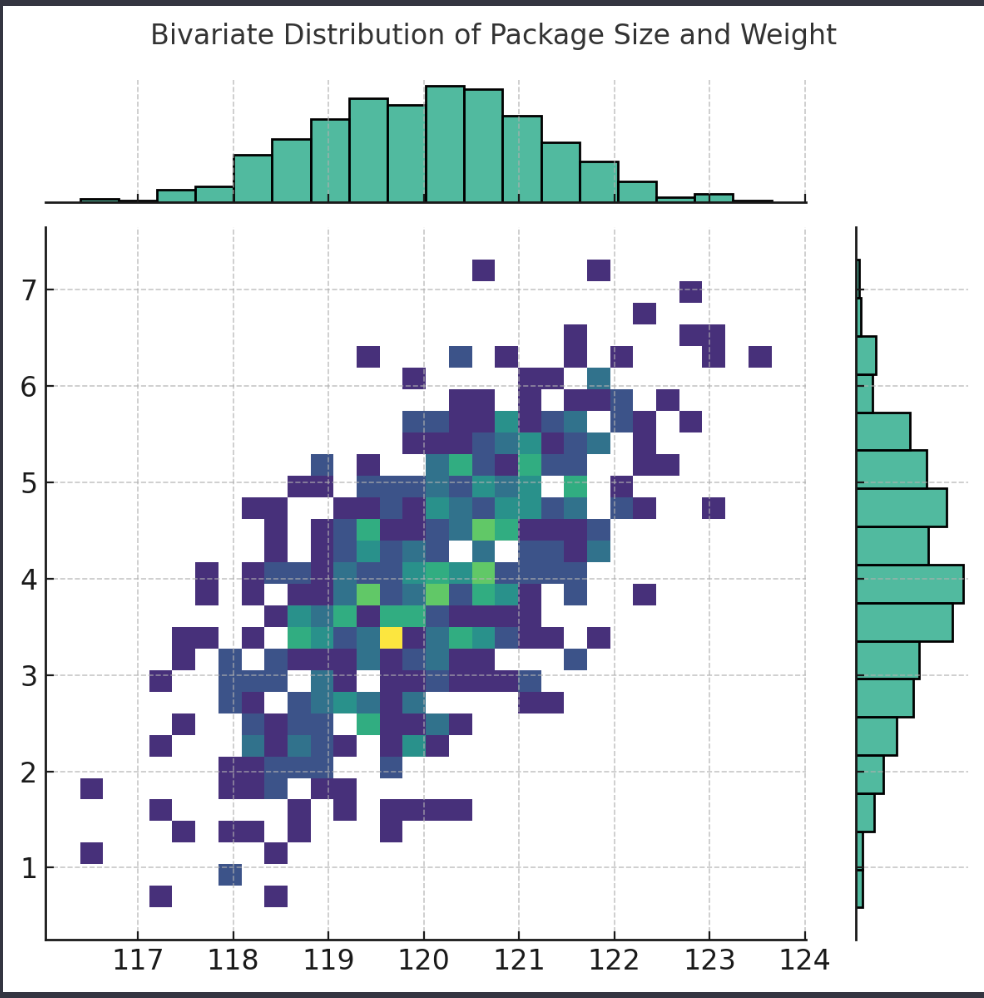
\includegraphics[width=0.5\linewidth]{a.png}
        \newline (b) After sampling 500 times from the joint Bivariate Gaussian distribution of package size \(S\) and weight \(W\), and plotting a bivariate histogram, the bin with the highest frequency corresponds to approximately \(S = 120\) in\(^3\) and \(W = 4\) pounds. Given the distribution parameters, \(\mu = \begin{bmatrix} 120 \\ 4 \end{bmatrix}\) and \(\Sigma = \begin{bmatrix} 1.5 & 1 \\ 1 & 1.5 \end{bmatrix}\), the theoretical expected values for size and weight are exactly \(S = 120\) in\(^3\) and \(W = 4\) pounds. The empirical values for the most likely combination of size and weight closely match the theoretical expectations of the given Bivariate Gaussian distribution.
        \ \newline 2. 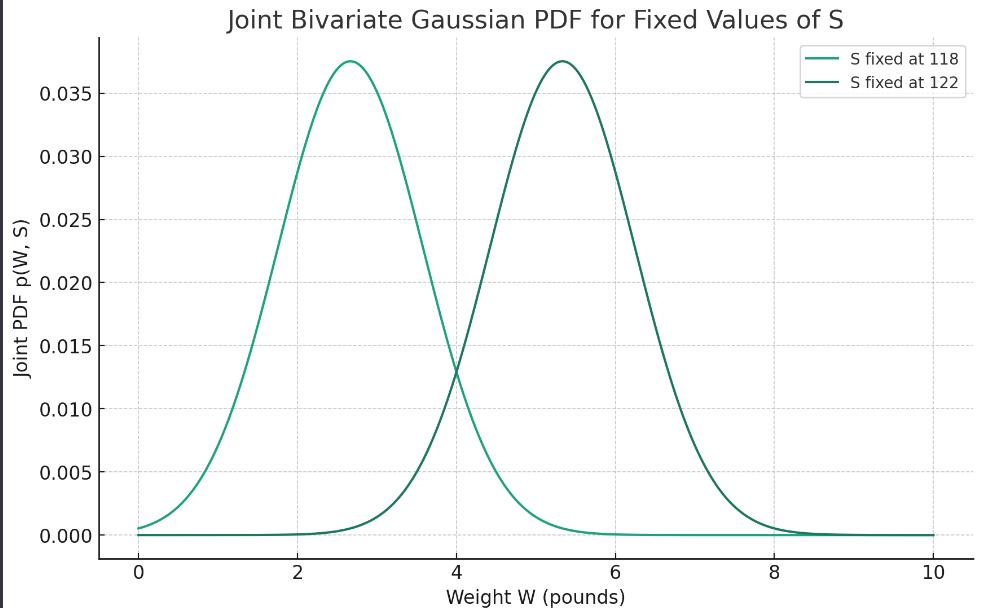
\includegraphics[width=0.5\linewidth]{b.png} The shift in the peak of the PDF for \(W\) as \(S\) changes from 118 to 122 illustrates a direct correlation: as \(S\) increases, the most likely value of \(W\) also increases. This demonstrates a positive correlation between \(S\) and \(W\), implying that larger packages tend to weigh more.
        \ \newline 3. The Gaussian distribution is appropriate for modeling the size and weight of packages due to the Central Limit Theorem, which suggests that the sum of many independent random variables tend to be normally distributed and thus reflect the aggregation of small, independent effects on package dimensions. It may also not be appropriate for similar reasons though, particularly for extreme values (outliers). Since real-world package sizes and weights can have hard boundaries (e.g., minimum and maximum limits) or skewed distributions, these are often not captured by the symmetric Gaussian model.
        \ \newline 4. Given \(T = 60 + 0.6W + 0.2S + \varepsilon\), where \(\varepsilon \sim N(0,5)\), \(W\) and \(S\) have a joint Gaussian distribution with means \(\mu_W = 4\), \(\mu_S = 120\), and \(\Sigma = \left[ \begin{array}{cc} 1.5 & 1 \\ 1 & 1.5 \end{array} \right]\), the expectation \(E(T)\) and variance \(Var(T)\) can be computed as follows:

The expectation of \(T\) is:
\[
E(T) = E(60) + E(0.6W) + E(0.2S) + E(\varepsilon) = 60 + 0.6E(W) + 0.2E(S) + E(\varepsilon)
\]
Given \(E(W) = 4\), \(E(S) = 120\), and \(E(\varepsilon) = 0\), we get:
\[
E(T) = 60 + 0.6 \times 4 + 0.2 \times 120 = 60 + 2.4 + 24 = 86.4
\]

The variance of \(T\) is:
\[
Var(T) = Var(60) + Var(0.6W) + Var(0.2S) + Var(\varepsilon) = 0 + 0.6^2Var(W) + 0.2^2Var(S) + Var(\varepsilon)
\]
Given \(Var(W) = 1.5\), \(Var(S) = 1.5\), and \(Var(\varepsilon) = 5\), we find:
\[
Var(T) = 0.6^2 \times 1.5 + 0.2^2 \times 1.5 + 5 = 0.54 + 0.06 + 5 = 5.6
\]

Thus, \(E(T) = 86.4\) seconds and \(Var(T) = 5.6\) seconds\(^2\).

\ \newline 5. see attached code 



\end{solution} 


\end{document}